\chapter{Robotersysteme}


Ein bis zwei  zur Einleitung des Kapitels...

%\begin{equation}
%sljdsjuhd = luhsdfiuhsf+ spidhfos
%\end{equation}


\section{PR2}

Der PR2 (Willow Garage Inc., Menlo Park, USA) ist ein \textbf{\textit{menschen�hnlicher} }Serviceroboter, der seinen Dienst in Wohnr�umen verrichten soll und derzeit im sogenannten PR2 Beta-Programm von elf Forschungseinrichtungen �ber einen Zeitraum von zwei Jahren getestet wird \cite{WillowGarage2010}.\\

\begin{figure}[!ht]
	\begin{center}
	\subfigure[]{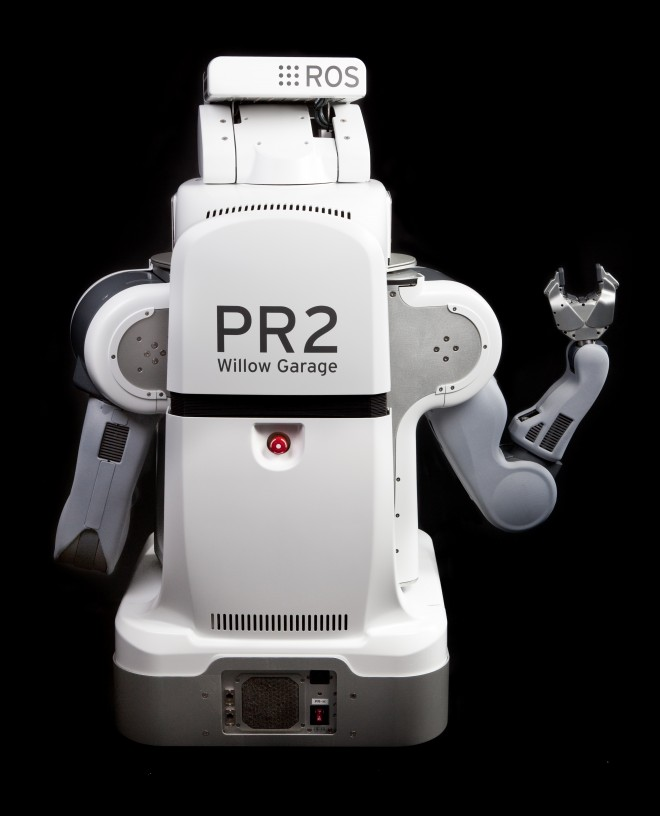
\includegraphics[height=45mm]{PR2-1}}
	\hspace{5mm}
	\subfigure[]{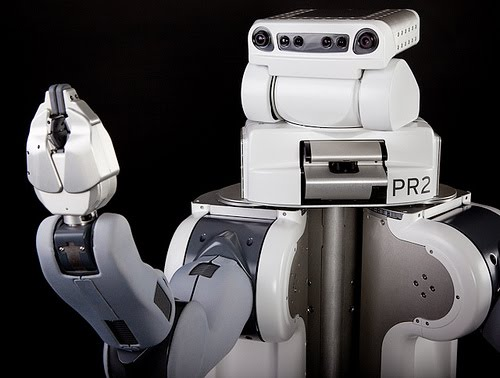
\includegraphics[height=45mm]{PR2-2}}
	\hspace{5mm}
	\subfigure[]{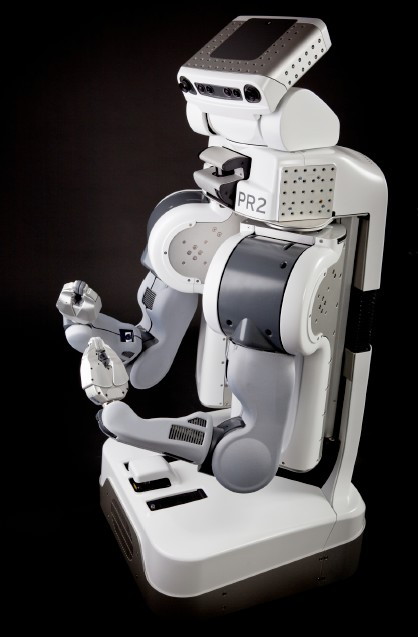
\includegraphics[height=45mm]{PR2-3}}
	\caption{PR2-Roboter (Quelle: Willow Garage)}
	\label{fig.PR2}
	\end{center}
	\vspace*{-8mm}
\end{figure}




Ausgestattet ist der PR2 mit zwei Armen, die jeweils sieben Freiheitsgrade haben und an deren Enden ein Greifer montiert ist, siehe \bild{PR2}. Die Sensorik des Armes besteht aus einer Kamera am Unterarm und Druck- sowie Beschleunigungssensoren am Greifer. Die Nutzlast eines Arms ist mit \SI{1,8}{\kilo\gram} ausgewiesen. Weiterhin verf�gt der Roboter �ber einen dreh- und schwenkbaren Kopf, in dem eine 5-Megapixel Farbkamera, ein LED-Texturprojektor und zwei Stereokameras integriert sind, wobei eine Kamera f�r die Fernsicht und die andere f�r die Objektmanipulation genutzt wird. Unterhalb des Kopfes ist ein schwenkbarer Laserscanner und ein Inertialsensor verbaut. Die Position des Oberk�rpers l�sst sich in der H�he zwischen \SI{1330}{\milli\meter} und \SI{1645}{\milli\meter} (Gesamth�he) variieren. Angetrieben wird die omnidirektionale Basis von vier gelenkten R�dern, die eine maximale Geschwindigkeit von \SI{3,6}{\kilo\meter\per\hour} erm�glichen. Die quadratische Basis hat eine Kantenl�nge von \SI{668}{\milli\meter}. Als Recheneinheit stehen zwei Server zur Verf�gung, die jeweils auf acht CPU-Kernen rechnen und dabei auf 24\,GB Arbeitsspeicher zugreifen k�nnen. Als Betriebssystem wird Ubuntu verwendet, auf dem das Robot Operating System, kurz ROS, die Grundlage f�r die Datenverarbeitung bildet. Da ROS innerhalb dieser Arbeit ebenfalls zum Einsatz kommt, wird dieses in \Sec{IntroductionROS} vorgestellt und an den entsprechenden Stellen weiter erl�utert. Die Kosten f�r einen PR2-Roboter belaufen sich derzeit auf etwa \SI{400.000}{US-Dollar}\footnotemark. Mit Hilfe des PR2 wurden von den zuvor erw�hnten Beta-Testern Szenarien bew�ltigt, die innerhalb des menschlichen Wohnraumes auftreten k�nnen. An der TU M�nchen hat ein PR2-Roboter beispielsweise zusammen mit einem anderen Robotersystem einen Pfannkuchen gebacken \cite{TUM2011}.
\footnotetext{Der angegebene Preis wurde am 16.08.2011 der Website http://www.willowgarage.com/pages/pr2/order entnommen und versteht sich exklusive Steuern und Versandkosten.}

\section{Technische Daten der youBot-Plattform}

\begin{table}[ht]
	\centering
	\caption{Technische Daten der youBot Plattform}\label{tab.TechSpecYouBotBase}
	\vspace*{-3mm}
	\begin{longtable}[ht]{|l|c|r|}\hline
		\rowcolor{Snow2}
		Bezeichnung						& Formelzeichen	& \\ \hline
		Gesamtl�nge 					&			& \SI{530}{\milli\meter}				\\ \hline
		Gesamtbreite 					&  		& \SI{350}{\milli\meter}				\\ \hline
		H�he									&  		& \SI{106}{\milli\meter}				\\ \hline
		Radstand							& $l$	& \SI{470}{\milli\meter}				\\
		\hline
	\end{longtable} 
	\vspace*{-3mm}
\end{table}


\begin{lstlisting}[label=source.launchHokuyo,caption=Launchfile zum Start der hokuyo\_node]
<!-- launch hokuyo node -->
<node pkg="hokuyo_node" type="hokuyo_node" name="hokuyo_node" output="screen">
	<param name="port" value="/dev/ttyACM0"/>
	<param name="frame_id" value="/base_laser_front_link"/>
</node>
\end{lstlisting}